% Evans second edition, section 3.1.
% English source: printed p. 90; PDF page 107 (1-based).
% Chinese section starts: checked against the chapter-opening list, PDF p. 79.
% Status: editorial study draft with detailed proofs and mathematical notes; no independent review.
\Needspace{65mm}
\section{Complete Integrals, Envelopes}
\label{sec:3-1}

\subsection{Complete integrals (Evans \S3.1.1)}
An $n$-parameter family $u(x;a)$ is a complete integral for
$F(Du,u,x)=0$ in $n$ independent variables if every member solves the
PDE and the $n\times(n+1)$ matrix
\[
 \bigl(D_a u,\ D^2_{ax}u\bigr)
\]
has rank $n$. The condition concerns variation of the whole first jet,
not only the gradient.
\Needspace{45mm}
\PDEAnnotation{完全积分不是所有解}{它是含足够独立参数的一族解，不能把“完全”理解成已经穷尽全部解。边界值通常是一整个函数，有限多个常数不能直接编码任意边界数据。}
If this family factored through $n-1$ parameters, $u(x;a)=v(x;\psi(a))$,
the chain rule would factor the displayed matrix through $D_a\psi$,
whose rank is at most $n-1$. Thus full rank rules out that redundancy.

\paragraph{Three useful families.}
For Clairaut's equation $x\cdot Du+f(Du)=u$,
\[
 u(x;a)=a\cdot x+f(a)
\]
solves the PDE and $D^2_{ax}u=I$, proving full rank.
For the eikonal equation $|Du|=1$, use $u=a\cdot x+b$ with $|a|=1$.
A local chart of the sphere has $n-1$ independent parameters and $b$
adds one; the independent tangential gradient variations and value
variation give rank $n$. This family is locally parametrized by an
open subset of $\R^n$, rather than treating the sphere as an open set.

For $u_t+H(D_xu)=0$ in $n+1$ independent variables,
\[
 u(x,t;a,b)=a\cdot x-tH(a)+b.
\]
There are $n+1$ parameters. The $a$ derivatives change $D_xu$ by the
standard basis, and the $b$ derivative changes the value by one
without changing the gradient. The corresponding jet matrix has
rank $n+1$, as required.

\subsection{Envelopes and singular integrals (Evans \S3.1.2, Theorem 1)}
\begin{theorem}\label{thm:3-envelope}
Let $U(x;a)$ be a smooth family of solutions and suppose
$D_aU(x;\alpha(x))=0$ with $\alpha$ continuously differentiable.
Then $v(x)=U(x;\alpha(x))$ is also a solution wherever this construction
is defined.
\end{theorem}
\begin{expandedproof}
For each coordinate, the full chain rule is
\[
 \partial_i v
 =\partial_{x_i}U(x;\alpha(x))
   +\sum_j\partial_{a_j}U(x;\alpha(x))\partial_i\alpha_j.
\]
The sum vanishes by the stationary-parameter condition. Thus $v$ and
the selected family member have the same value and the same spatial
gradient at $x$. Substitution into $F$ proves the PDE.
To obtain a smooth stationary parameter locally, one sufficient condition
is invertibility of $D^2_{aa}U$, by the implicit function theorem.
That condition is sufficient, not part of the abstract envelope identity.
\end{expandedproof}
\Needspace{45mm}
\PDEAnnotation{为何参数导数消失}{对 $U(x,\alpha(x))$ 求导时，不能忘掉参数链式项。正是 $D_aU=0$ 使它消失，包络与被选中的曲面才在该点相切。}

For $U(x,t;a)=a\cdot x-t|a|^2$, stationarity gives $a=x/(2t)$,
and the envelope is $v(x,t)=|x|^2/(4t)$ for $t>0$.
Indeed $v_t=-|x|^2/(4t^2)$ and $|D_xv|^2=|x|^2/(4t^2)$.
This example uses $H(p)=|p|^2$; later the common choice $H=|p|^2/2$
has a different factor of two.
\Needspace{45mm}
\PDEAnnotation{二次 Hamiltonian 的系数}{若 $H(p)=|p|^2$，其对偶为 $L(v)=|v|^2/4$；若 $H(p)=|p|^2/2$，则 $L(v)=|v|^2/2$。检查公式时，把 PDE、对偶与包络中的系数一起核对。}

For $U(x;a)=\pm\sqrt{1-|x-a|^2}$, the PDE is
$U^2(1+|DU|^2)=1$. Stationarity yields $a=x$ and the envelopes
$v=\pm1$. The derivative with respect to $a$ of the upper branch is
$(x-a)/\sqrt{1-|x-a|^2}$; changing the branch changes the sign.

One can restrict the parameters to $a=(a',h(a'))$ and then form an
envelope over $a'$. The stationary equations become
$U_{a_i}+U_{a_n}h_{a_i}=0$. The resulting general integral depends on
the arbitrary function $h$, whenever a smooth envelope exists.
It still need not describe every PDE solution: a factorized equation
$F_1(Du,u,x)F_2(Du,u,x)=0$ may have a branch belonging only to $F_2$.

\begin{center}
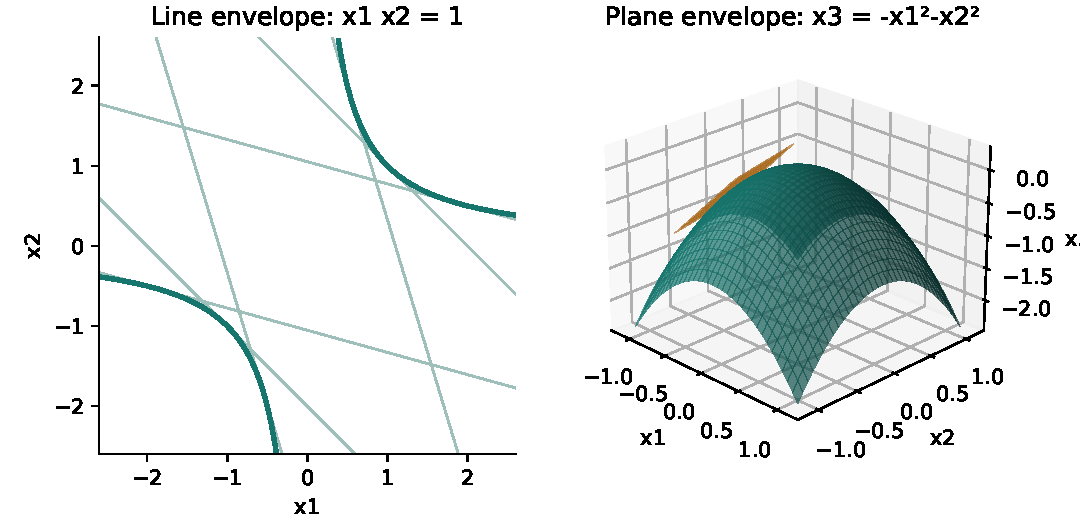
\includegraphics[width=\linewidth]{output/figures/ch03-envelopes.pdf}
\end{center}
\noindent\textit{Editorial figure for Problem 2.}
A hyperbola is tangent to a family of lines; a negative paraboloid
is tangent to the associated family of planes. Elimination and
parameter-domain restrictions are worked out in the exercise solution.
